\subsection{Perceptron}

\begin{frame}
\frametitle{Perceptron}

\begin{columns}

\column{0.45\textwidth}
\begin{itemize}
\item Ähnliche Aktivierungsfunktion wie beim MP-Neuron
\item Jedoch gewichtete kontinuierliche Eingabewerte
\end{itemize}


\column{0.4\textwidth}
\begin{figure}
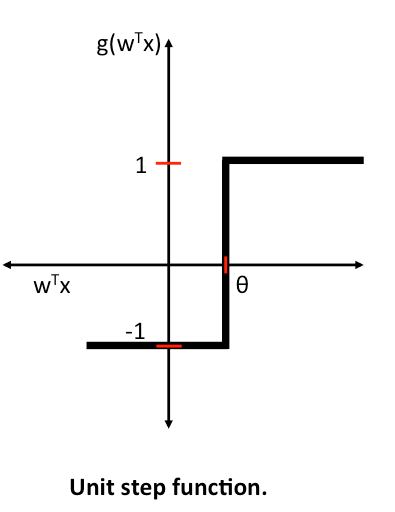
\includegraphics[width=.8\linewidth]{./geschichtliches/perceptron/img/perceptron_einheitsSprungfunktion_alpha}
\end{figure}

\end{columns}


\hspace{1mm}
\hrule


\begin{columns}

\column{0.4\textwidth}
\begin{align*} 
\mathbf{w} = \begin{bmatrix}
    w_{1}  \\
    \vdots \\
    w_{m}
\end{bmatrix}
\quad  \mathbf{x} = \begin{bmatrix}
    x_{1}  \\
    \vdots \\
    x_{m}
\end{bmatrix}
\end{align*}

\column{0.4\textwidth}
\begin{align*}
\begin{split}
z & =  w_1x_{1} + \dots + w_mx_{m} \\
 & = \sum_{j=1}^{m} x_{j}w_{j} \\
 & = \mathbf{w}^T\mathbf{x}
\end{split}
\end{align*}
\end{columns}
\end{frame}


\begin{frame}
\frametitle{Aufbau}

\begin{figure}
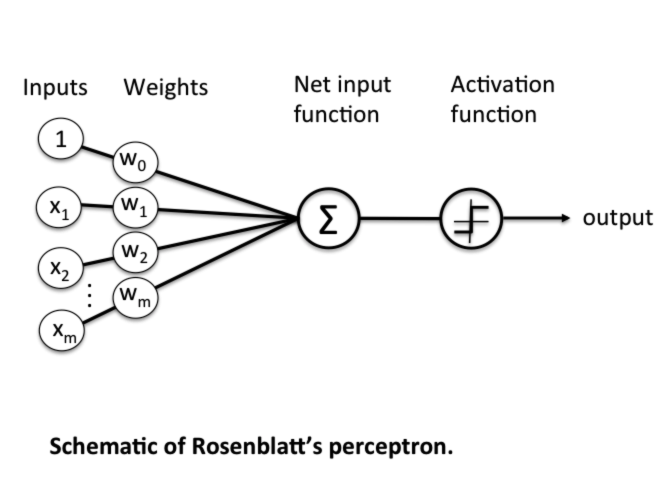
\includegraphics[width=.6\linewidth]{./geschichtliches/perceptron/img/perceptron_schematisch_alpha}
\end{figure}


\hrule


\begin{columns}

\column{0.4\textwidth}
\begin{align*}
g(z) =\begin{cases}
	0 & \mbox{if } z \leq 0 \\
    1 & \mbox{if } z > 0
  \end{cases}
\end{align*}
\vspace{1mm}

\column{0.4\textwidth}
\begin{align*}
\begin{split}
z & = \mathbf{w_0x_{0}} + w_1x_{1} + \dots + w_mx_{m} \\
 & = \sum_{j=0}^{m} x_{j}w_{j} \\
 & = w^Tx
\end{split}
\end{align*}

\end{columns}

\end{frame}


\begin{frame}
\frametitle{Lernregel - Ablauf}

\begin{itemize}
\item Modell übernimmt selbst die Anpassung der Gewichte
\item Test mittels einer Menge von gelabelten Trainingsdatensätzen
\end{itemize}
\hspace{1mm}

\begin{block}{Grober Ablauf}
\begin{itemize}
\item Initialisiere die Gewichte mit einem sehr kleinen Wert oder 0.
\item Für jeden Datensatz der Menge von Trainingsdatensätzen:
\begin{itemize}
	\item Berechne den Ausgabewert des Systems
	\item Gleiche die Gewichte an
\end{itemize}
\end{itemize}
\end{block}

\end{frame}


\begin{frame}
\frametitle{Lernregel - Formel}

\begin{block}{Angleichung der Gewichte}
\begin{itemize}
\item Gewichte komponentenweise angleichen: $w_j := w_j + \Delta w_j$
\item Gewichtsänderung: $\Delta w_j = \eta \; (\text{target}^{(i)} - \text{output}^{(i)})\;x^{(i)}_{j}$
\end{itemize}
\end{block}

\begin{itemize}
\item Beispiel - Iteration mit zweidimensionalem Trainingsvektor:
\begin{align*}
\begin{aligned}
& \Delta w_0 = \eta(\text{target}^{(i)} - \text{output}^{(i)}) \\
& \Delta w_1 = \eta(\text{target}^{(i)} - \text{output}^{(i)})\;x^{(i)}_{1} \\
& \Delta w_2 = \eta(\text{target}^{(i)} - \text{output}^{(i)})\;x^{(i)}_{2}
\end{aligned}
\end{align*}
\end{itemize}
\end{frame}


\begin{frame}
\frametitle{Lernregel - Trainingsbeispiele}

\begin{itemize}
\item Trainingsdatensatz richtig erkannt: 
\begin{align*}
\begin{aligned}
& \Delta w_j = \eta(1^{(i)} - 1^{(i)})\;x^{(i)}_{j} = 0 \\
& \Delta w_j = \eta(1^{(i)} - 1^{(i)})\;x^{(i)}_{j} = 0 \\
\end{aligned}
\end{align*}

\item Trainingsdatensatz falsch erkannt:
\begin{align*}
\begin{aligned}
& \Delta w_j = \eta(1^{(i)} - -1^{(i)})\;x^{(i)}_{j} = \eta(2)\;x^{(i)}_{j} \\
& \Delta w_j = \eta(-1^{(i)} - 1^{(i)})\;x^{(i)}_{j} = \eta(-2)\;x^{(i)}_{j} \\
\end{aligned}
\end{align*}

\end{itemize}
\end{frame}


